\documentclass{sig-alternate}
 



% Use this command to override the default ACM copyright statement (e.g. for preprints).
% Consult the conference website for the camera-ready copyright statement.


%% EXAMPLE BEGIN -- HOW TO OVERRIDE THE DEFAULT COPYRIGHT STRIP -- (July 22, 2013 - Paul Baumann)
 %\toappear{Permission to make digital or hard copies of all or part of this work for personal or classroom use is 	granted without fee provided that copies are not made or distributed for profit or commercial advantage and that copies bear this notice and the full citation on the first page. Copyrights for components of this work owned by others than ACM must be honored. Abstracting with credit is permitted. To copy otherwise, or republish, to post on servers or to redistribute to lists, requires prior specific permission and/or a fee. Request permissions from permissions@acm.org. \\
% {\emph{BuildSys'16}}, Nov 16--17, 2014, Stanford,California USA. \\
% Copyright \copyright~2016 ACM ISBN/14/04...\$15.00. \\
% DOI string from ACM form confirmation}
%% EXAMPLE END -- HOW TO OVERRIDE THE DEFAULT COPYRIGHT STRIP -- (July 22, 2013 - Paul Baumann)


% Arabic page numbers for submission.
% Remove this line to eliminate page numbers for the camera ready copy
\pagenumbering{arabic}


% Load basic packages
\usepackage{balance}  % to better equalize the last page
\usepackage{graphics} % for EPS, load graphicx instead
\usepackage{times}    % comment if you want LaTeX's default font
\usepackage{url}      % llt: nicely formatted URLs
\usepackage{epic,epsfig}
\usepackage{wrapfig}
 \usepackage{graphicx}
\usepackage[caption = false]{subfig}
\usepackage{float}
\usepackage{verbatim}
 

% llt: Define a global style for URLs, rather that the default one
\makeatletter
\def\url@leostyle{%
  \@ifundefined{selectfont}{\def\UrlFont{\sf}}{\def\UrlFont{\small\bf\ttfamily}}}
\makeatother
\urlstyle{leo}


% To make various LaTeX processors do the right thing with page size.
\def\pprw{8.5in}
\def\pprh{11in}
\special{papersize=\pprw,\pprh}
\setlength{\paperwidth}{\pprw}
\setlength{\paperheight}{\pprh}
\setlength{\pdfpagewidth}{\pprw}
\setlength{\pdfpageheight}{\pprh}

% Make sure hyperref comes last of your loaded packages,
% to give it a fighting chance of not being over-written,
% since its job is to redefine many LaTeX commands.
\usepackage[pdftex]{hyperref}
\hypersetup{
pdftitle={SIGCHI Conference Proceedings Format},
pdfauthor={LaTeX},
pdfkeywords={SIGCHI, proceedings, archival format},
bookmarksnumbered,
pdfstartview={FitH},
colorlinks,
citecolor=black,
filecolor=black,
linkcolor=black,
urlcolor=black,
breaklinks=true,
}

% create a shortcut to typeset table headings
\newcommand\tabhead[1]{\small\textbf{#1}}


% End of preamble. Here it comes the document.
\begin{document}
 

%\title{Activity-Aware Identification of Fine-grained Appliance Usage for Green Buildings}
\title{Low Cost Thermal Imaging System for Monitoring Building Insulation}
%\numberofauthors{3}
%\author{
%  \alignauthor Nilavra Pathak\\
%    \affaddr{Information Systems}\\
%    \affaddr{University of Maryland Baltimore County}\\
%    \email{nilavra1@umbc.edu}\\ 
%    %\affaddr{Optional phone numbe00r} 
%}

\maketitle

\begin{abstract}
   Thermal Imaging helps detect air leakages, uneven heating or cooling pockets, and damped walls in building environments. For detection of such unseen insulation problems, we present a Thermal Imagery system that captures heat signatures of wall surfaces and provides an integrated thermal image of an entire room. In this paper, we build an alternative compared to the expensive commercially available circuit module consisting of an IR camera connected to a micro-controller with I$^2$C communication protocol, by a Raspberry-Pi module, to reduce the cost of existing thermal imaging system by an order of magnitude. The unit is capable of rotating automatically in pre-calibrated angle and capturing surface thermal images of 16 $\times$ 4 resolution which are then run by an Image Stitching technique to produce an integrated thermal image of the wall surfaces. Finally, another camera unit is placed in-situ to capture the digital images of the wall surface to combine with the reconstructed thermal images to get an overall high-resolution thermal layout of the wall surfaces. The proposed system, based on our preliminary studies, is proven to be a cost effective and user friendly system to detect building leakages, damps and irregular heating/ cooling losses.
\end{abstract}

\section{Introduction} 

 \indent Building structures, openings and leakages have direct effect on the heating and cooling of homes. Often it has been found that the utility bill is exorbitantly high. Maryland has one of the highest bills in USA~\cite{EIA2014}, where the average monthly utility bill is about \$140. Typically utility costs go up in winter and mostly during bouts of bitter cold when more people are likely to stay indoors HVAC usage spikes up. Times like the winter storm which disrupts may result in families to stay indoors for more number of days hence increasing utility consumption. As such proper heating in the house is a requisite and minimizing the heat loss is necessary to reduce utility bills and also for comfort. Structural openings and leakages can result in uneven thermal pockets in a room or house. Slight openings in doors and windows can be major reasons for heat leakages which can be detected using thermal imagery. Apart from that infrared building diagnosis provides detection of - water leaks and their origin - walls, flooring, roof; plumbing issues like blockages; electrical "hot spots" which can cause potential fire hazards; Pest \& rodent nests; Moisture that cannot be physically reached with moisture meters; HVAC problem areas - loose, ill-fitting or disconnected fittings. However diagnosis providers or self-diagnosis using IR cameras needs manual searching of leakages and uses expensive thermal imaging devices. 
  
 \indent Our system description is somewhat similar to SPOT+~\cite{SPOT,SPOT+} although our intention and the hardware is completely different. The SPOT system consist of a Kinect sensor, a Infrared Sensor and servo motor, along with environment sensors as the main objective of the system is occupancy based comfort management. The system is described as - "\textit{ When a worker enters the work space, the Kinect tracks the worker and sends a skeleton stream to the PC. The PC finds the location of the worker's body center and calculates the rotation angle of the servos. It then communicates with the micro-controller to adjust the angle of the two servos so that the infrared sensor is facing the body center. When the tracked worker is moving, the infrared sensor may not be actually facing towards the worker. Therefore, we introduce a 0.5 second measurement delay into the system. That is, the infrared sensor starts collecting data only when the worker has been standing still for at least 0.5s. The system then estimates the clothing insulation by the clothing surface temperature ..}". 

\indent Technical Questions: Our investigations in this paper address the following technical questions:
 \begin{itemize}
 \item The commercially available imaging systems are expensive and range from \$250 upwards upto almost \$40000. Although such an expensive system is not necessary even the ones on low range are expensive. The IR research module also has an expensive board which cost \$170.
 
 \item We use an IR camera having a coarse resolution of 16 $\times$ 4 pixels. Calibration with the digital camera is a challenge and ground truth evaluation is difficult. From such a coarse resolution thermal image it is difficult to interpret what camera actually captures.
 
 \item The system in SPOT+ has a Kinect and IR sensor together. As such the system is quite cumbersome and not suitable for portable deployment. Also the cost goes high up with the Kinect attached. 
 \end{itemize}

 \indent \textbf{Key Contributions:} We believe that our innovations and results provide strong preliminary evidence that such a hybrid model, where low resolution thermal imagery is used to detect the several thermal sources, can prove to be an attractive and practically viable alternative for building leakage and occupancy detection. The key contributions of our work are as follows.
 
 \begin{itemize}
 \item We develop an integrated thermal imaging system which is capable of capturing snippets of thermal images of wall surfaces. The system can rotate automatically in a pre-calibrated angle to capture continuous IR snapshots in small offsets. The system also has a digital camera which captures images of wall surface.
 
 \item The second part of the system is the Image Reconstruction Unit. The IR images and the digital image is transferred to the external Image processing unit where the thermal images are stitched to get a panoramic image and then we detect - human body, cold surface and hot surface.
 \end{itemize}
 
 Rest of the paper is organized as follows. In Section 2 we present the overall architecture of the system. In Section 3 the different components of the imaging system and their detailed description.

\section{Overview}

\indent The overview of the system has been described in~\ref{fig:Overview}. The system has two major components - Complete Camera Module and the Image Processing Unit. The Complete Camera Module (CCM) consists of the IR camera, Digital camera and the Motor modules. All three modules are controlled by a Raspberry Pi. The motor rotates by a pre-calibrated angle and both the digital and infrared images are taken simultaneously and sent over to a PC where the Image Processing Unit (IPU) is present. The first task of IPU is pre-processing images and generate the heat maps for the thermal data. In the training phase the digital images are stitched together and the same stitching mechanism is applied for the IR images in testing phase. Processed images give the thermal layout of a wall surface which can be used for analytics. 

\begin{figure}[!h] 
\begin{center}
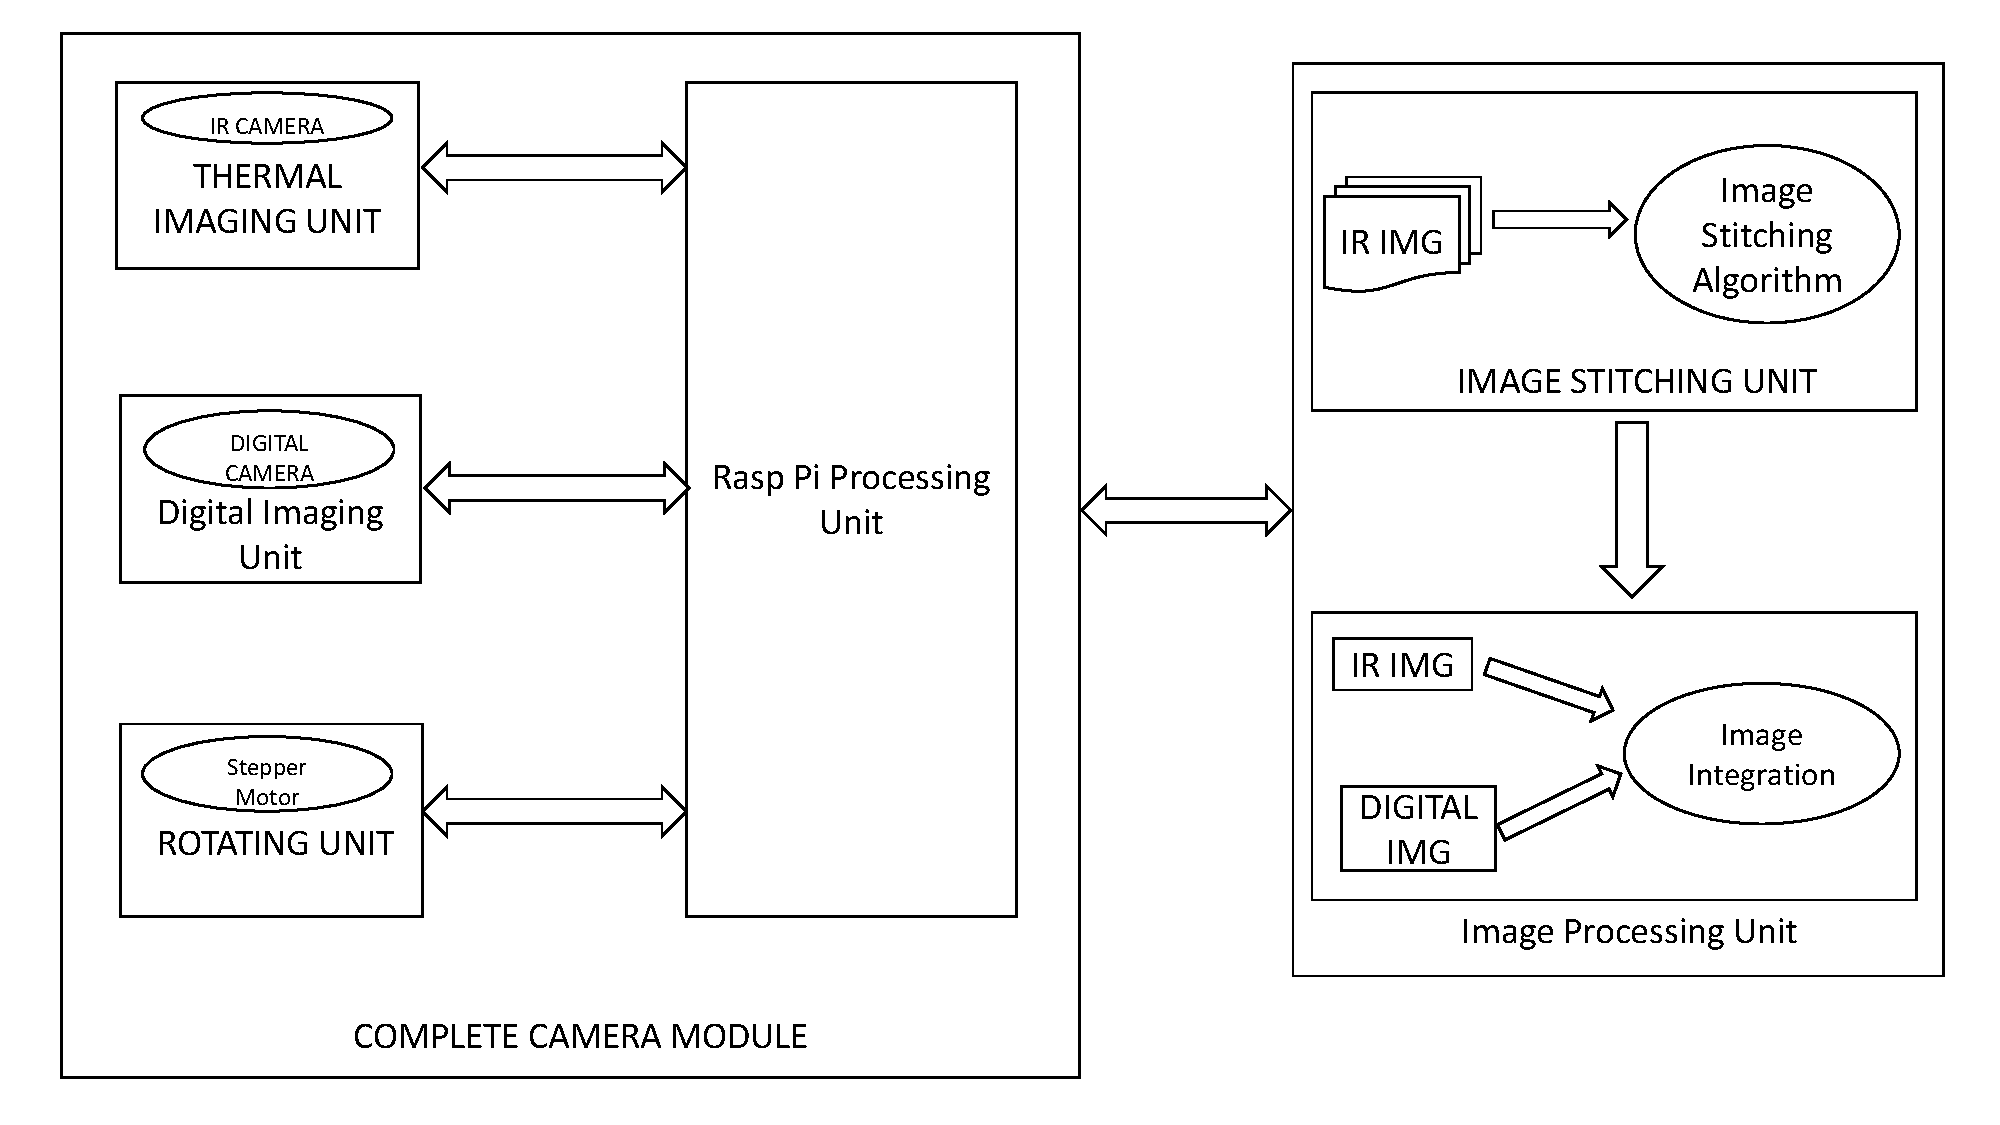
\epsfig{file=SystemBlockDIagram.pdf, height=1.5in,width=2.5in}
\vspace{-.1in}
 \caption{Thermal Imaging System Block Diagram}
 \label{fig:Overview}
\end{center}
\end{figure}

\section{Thermal Imaging System}

	In this section we describe the different components of the Thermal Imaging System. The overall block diagram of the system is shown in Figure~\ref{fig:Overview}. The two subsystems are the Complete Camera Module and the Image Processing Unit. In the following subsections the each of the subsystems are explained in details.
	\begin{figure}[!htb]
\begin{center}
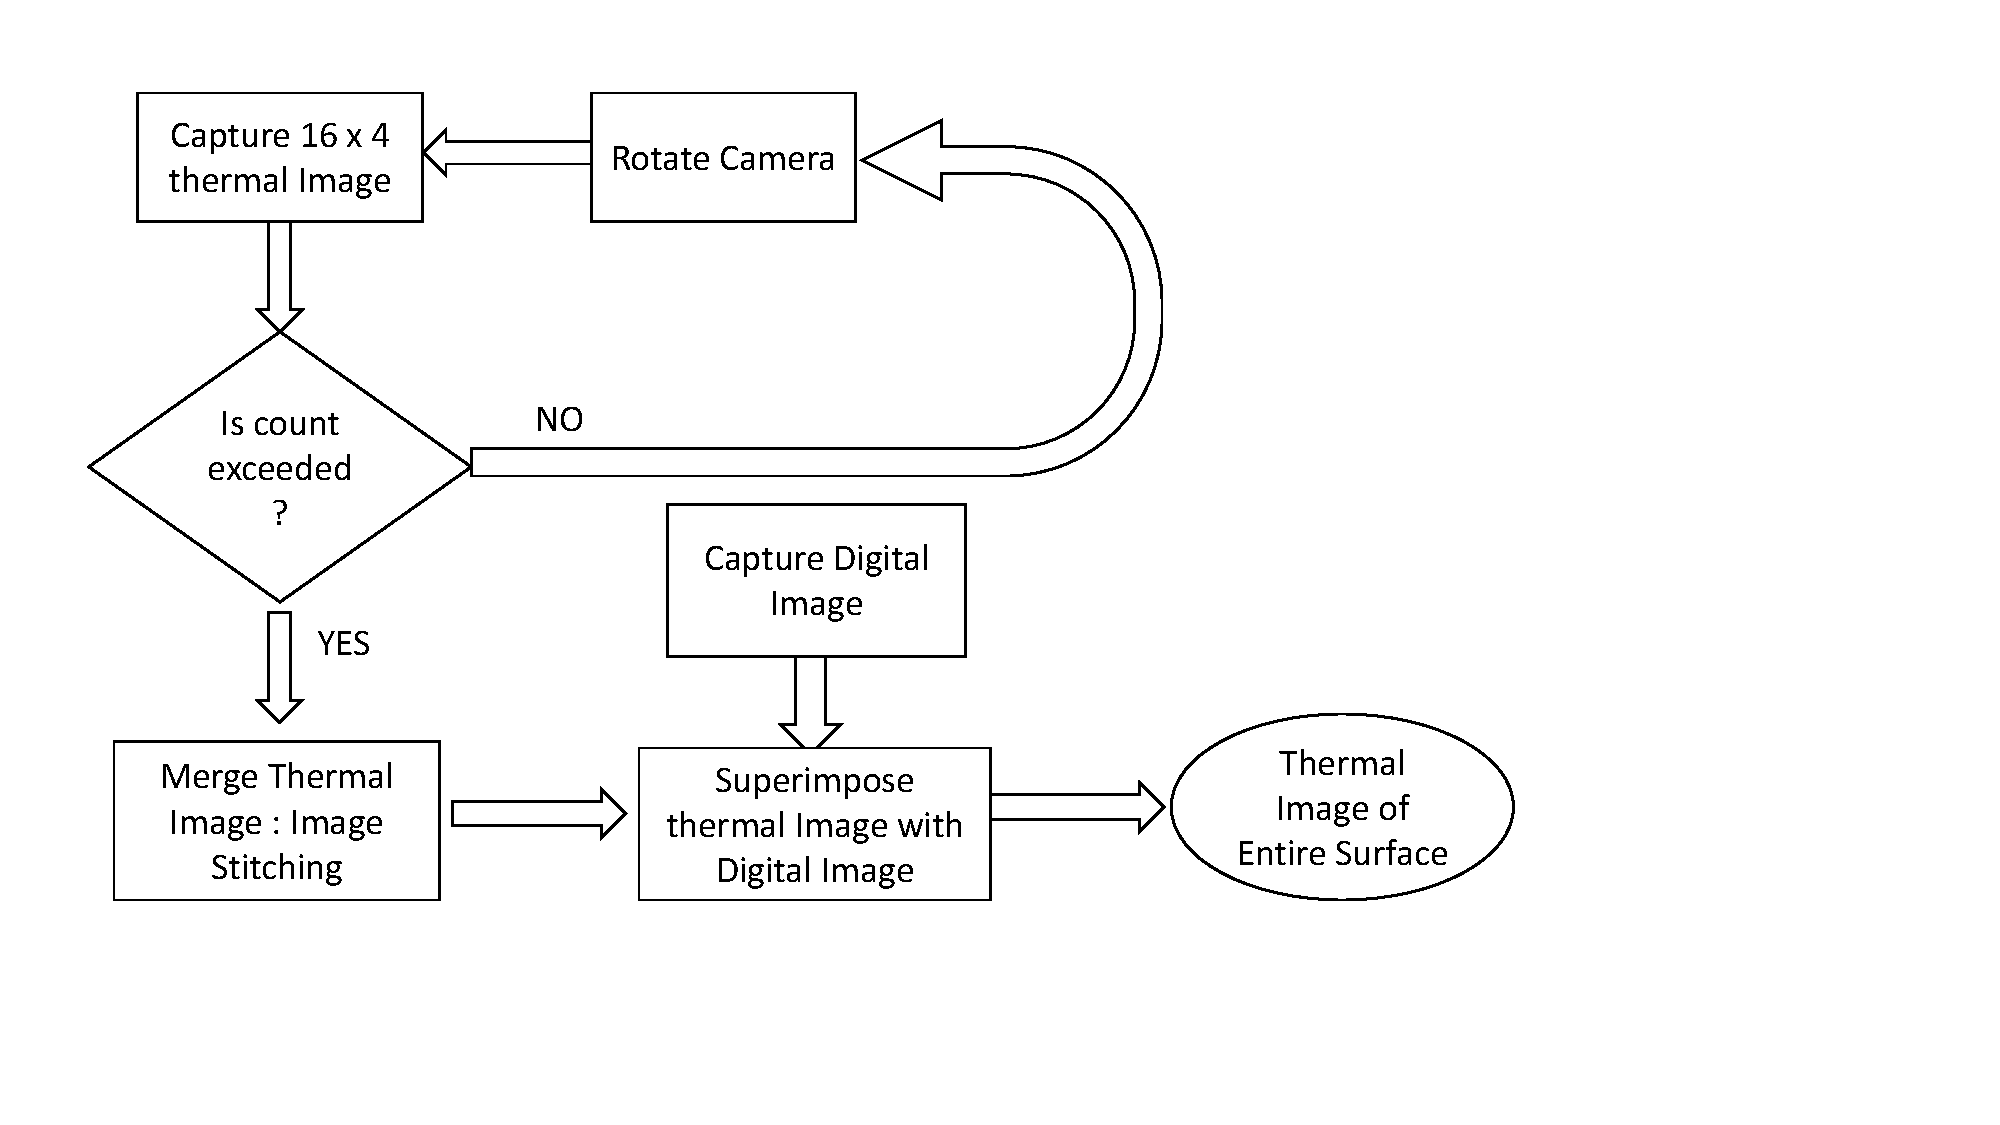
\epsfig{file=FlowDiagram.pdf, height=1.5in,width=2.5in}
 \caption{Thermal Imaging System Flow Diagram}
 \label{fig:Flow}
\end{center}
\end{figure}
	
	
	\subsection{Complete Camera Module}
	The camera module consist of the IR camera, which is controlled using the Raspberry pi. We use a MLX90621 IR camera which has a I$^2$C communication protocol. It detects background radiant temperature between -40$^{\circ}$C to +85$^{\circ}$C with a resolution of 0.02$^{\circ}$C and -50$^{\circ}$C to -300$^{\circ}$C for the object temperature. A raspberry pi camera is added 	The other part is a digital camera which is controlled by the Raspberry Pi. Both the digital and IR camera are attached to a circuit board in the same line. Figure~\ref{} is the circuit for the camera module.\\	
	\indent Module Rotation Unit is rotated by a stepper motor and controlled by the Raspberry Pi. The entire camera module is mounted on a (case) which can be rotated by the stepper motor. The stepper motor is calibrated to move at x$^{\circ}$ every xxxx seconds and capture the thermal images. A digital image of the wall surface is also taken and the stored. The data is stored in locally overtime and is transferred to server periodically.
	
	\subsection{Image Processing Unit}

	The image processing unit has two sections. The first part is the image stitching unit where the overlapping thermal images are stitched together to get a panorama like thermal image. Although this section is important but we don't invest much on algorithmic developments. After much survey of different available algorithms and tools we choose the Hugin tool for image stitching. If a sequence $I = \{I_1, I_2 ... I_n\}$  the stitched image $I_{sttich}$ is the panoramic image which we want to get. In Figure~\ref{fig:Individual} the individual images in a stream has been shown for the baseline images and the stitched image is shown in Figure~\ref{fig:Stitch} and thermal mask for the stitched image. The fridge and the heaters are shown in the image. Our assumption is under normal conditions there is no one around and all appliances are off, so when anyone moves in or a hot or cold surface shows up then the that will show up.\\	
	\indent Creating the thermal stitch image is simply a tricky manipulation if the tool. Merging the IR images is not possible instead we take help of the digital stitching to create the thermal panorama. After the digital stitch is constructed a project .pto file is created. Now if this .pto file is loaded in the tool again then it will search for the initial set of images used in the same folder. The trick is to replace these digital images with the corresponding thermal images. Although the thermal image offsets have not been aligned we get close results with thermal reconstruction. During the testing phase when an unknown set of thermal images are to be merged, we used the same .pto file for baseline digital image panorama construction for the new thermal reconstruction. When the two images are merged together the thermal mask is created for new images which identifies the open fridge or someone standing etc. One problem with the tool is during panorama construction is if someone moves the process fails. \\
	\indent Final part consist of merging the digital panoramic image with the thermal panoramic image. The process used is hybrid image construction, where the mask image or the thermal image is passed through a low pass filter and the digital image is passed through a high frequency filter and then the two images are combined. A complete procedure of the IPU have been described in Algorithm~\ref{algo:IPU}.


 
\begin{figure*}[!htp]  
  \begin{minipage}{0.16\textwidth}
\begin{center}
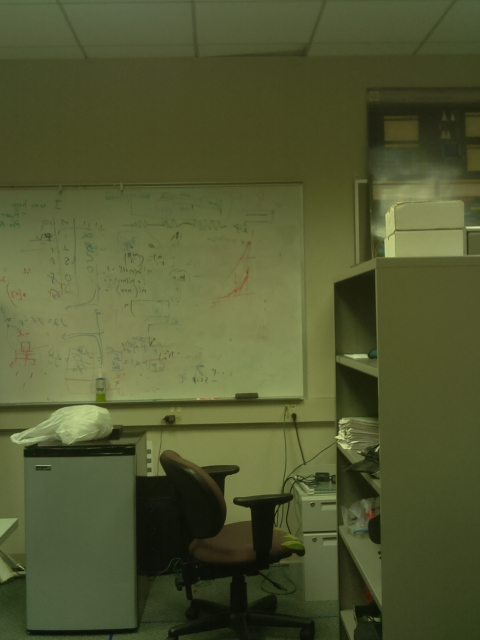
\epsfig{file=pic0.jpg,height=1in,width=1in}
 \end{center}
\end{minipage}
\begin{minipage}{0.16\textwidth}
\begin{center}
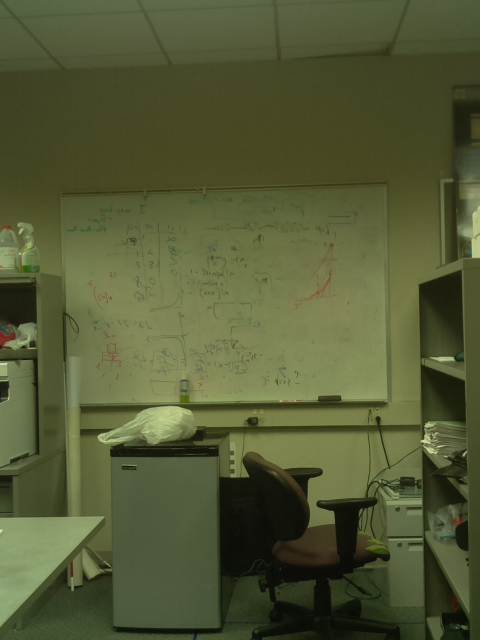
\epsfig{file=pic1.jpg,height=1in,width=1in}
 \end{center}
\end{minipage}
\begin{minipage}{0.16\textwidth}
\begin{center}
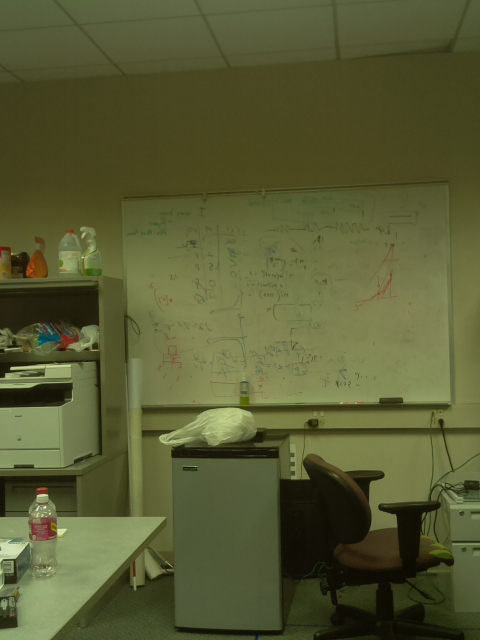
\epsfig{file=pic2.jpg,height=1in,width=1in}
 \end{center}
\end{minipage}
\begin{minipage}{0.16\textwidth}
\begin{center}
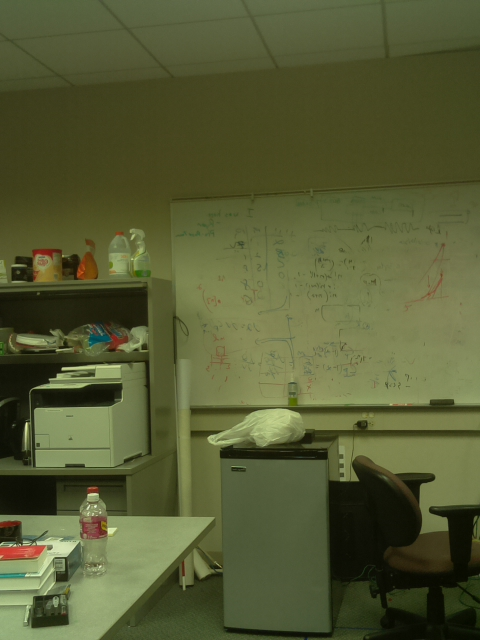
\epsfig{file=pic3.jpg,height=1in,width=1in}
 \end{center}
\end{minipage}
\begin{minipage}{0.16\textwidth}
\begin{center}
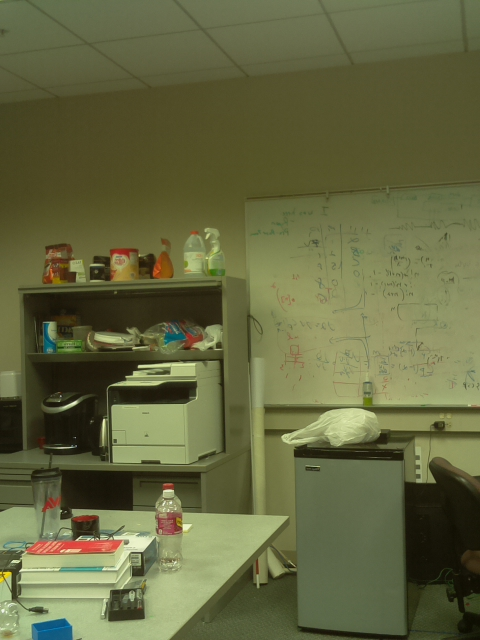
\epsfig{file=pic4.jpg,height=1in,width=1in}
 \end{center}
\end{minipage}
\begin{minipage}{0.16\textwidth}
\begin{center}
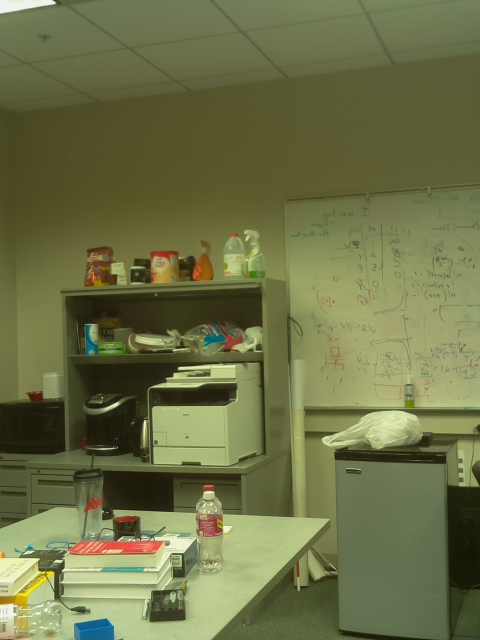
\epsfig{file=pic5.jpg,height=1in,width=1in}
 \end{center}
\end{minipage}
\begin{minipage}{0.16\textwidth}
\begin{center}
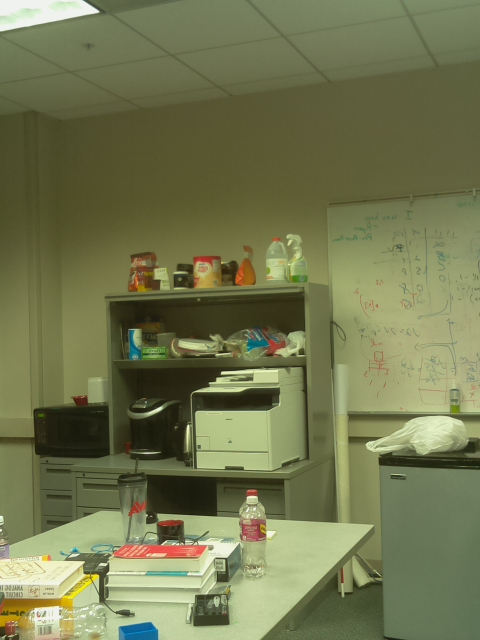
\epsfig{file=pic6.jpg,height=1in,width=1in}
 \end{center}
\end{minipage}
\begin{minipage}{0.16\textwidth}
\begin{center}
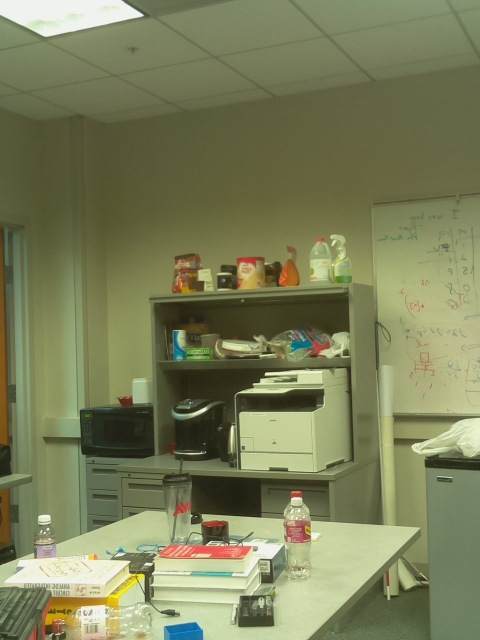
\epsfig{file=pic7.jpg,height=1in,width=1in}
 \end{center}
\end{minipage}
\begin{minipage}{0.16\textwidth}
\begin{center}
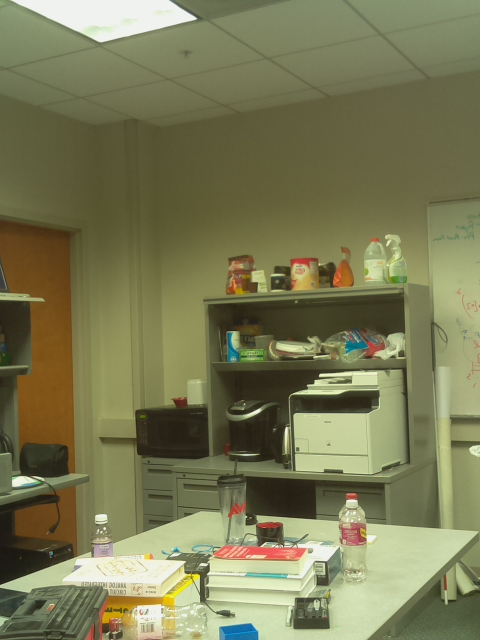
\epsfig{file=pic8.jpg,height=1in,width=1in}
 \end{center}
\end{minipage}
\begin{minipage}{0.16\textwidth}
\begin{center}
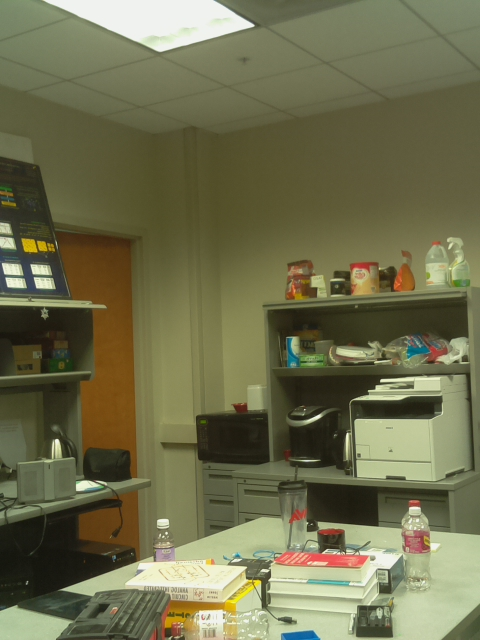
\epsfig{file=pic9.jpg,height=1in,width=1in}
 \end{center}
\end{minipage}
\begin{minipage}{0.16\textwidth}
\begin{center}
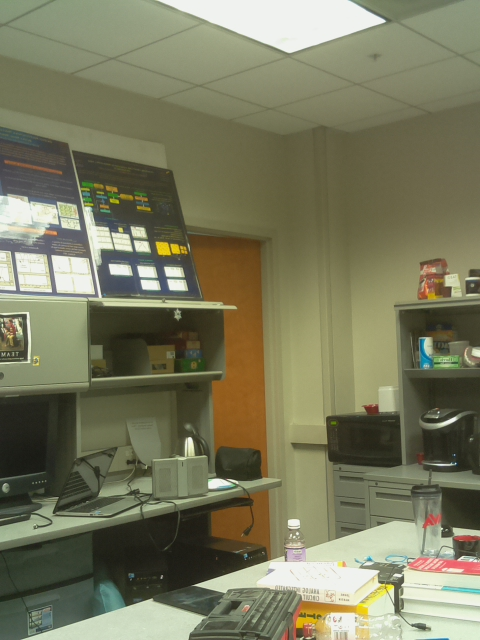
\epsfig{file=pic11.jpg,height=1in,width=1in}
 \end{center}
\end{minipage}
\begin{minipage}{0.16\textwidth}
\begin{center}
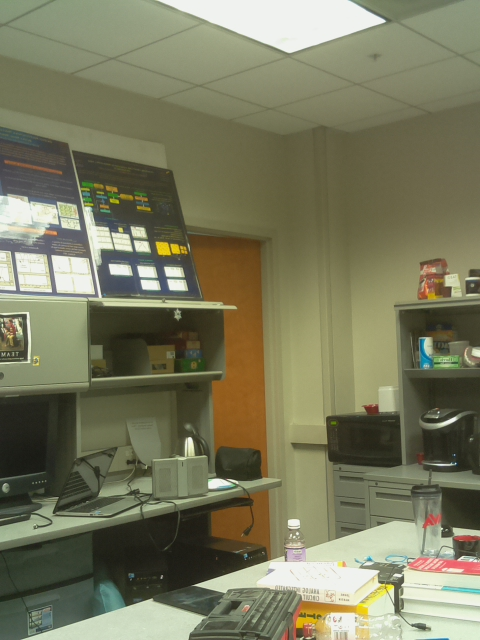
\epsfig{file=pic11.jpg,height=1in,width=1in}
 \end{center}
\end{minipage}
\caption{Baseline Stream of Images}
\label{fig:Individual}
\end{figure*}



\begin{figure*}[!htp] 
\begin{minipage}{0.01\textwidth}
\begin{center}
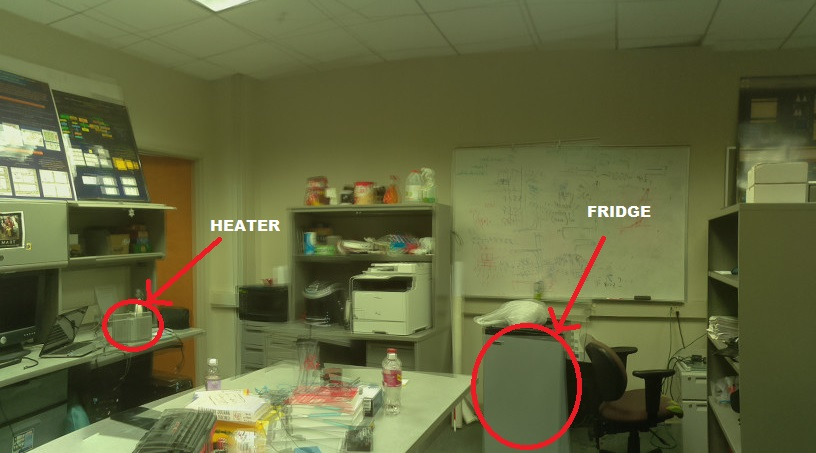
\epsfig{file=pic0pic11blendedfused.jpg,height=1.5in,width=2.5in}
\end{center}
\end{minipage}
\begin{minipage}{1.2\textwidth}
\begin{center}
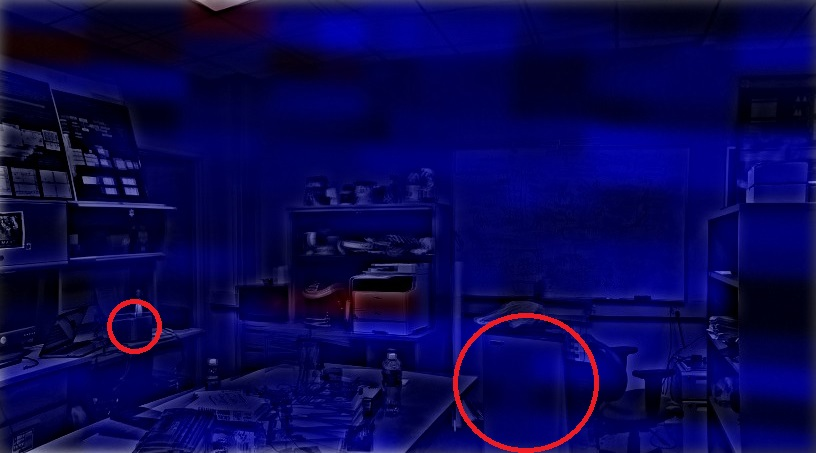
\epsfig{file=hybridimagescales.jpg,height=1.5in,width=2.5in }
\end{center}
\end{minipage}
\caption{Stitched Result for Baseline Stream of Images}
\label{fig:Stitch}
\end{figure*}
 

\begin{figure}[!htp]
\begin{minipage}{0.00\textwidth}
\mbox{}
\end{minipage}
\begin{minipage}{0.48\textwidth}
\begin{center}
\scriptsize{
\fbox{\parbox{5cm}{\texttt{
\begin{tabbing}
\=Procedure IPU(Input: \\Individual set of baseline digital images($D$) \\and corresponding thermal images ($I$) \\
\> Output: Thermal Panoramic Image\\
1. \= Create panoramic Image for the\\ baseline digital images using Hugin tool\\
2. \> Replace the digital images with the thermal images and\\ load the saved project again to construct the\\ panoramic thermal image\\
3. \> Use High pass filter on the digital image \\
4. \> Use Low pass filter on the IR image \\
5. \> Combine the two to get masked thermal image
\end{tabbing}}}}}
\caption{IPU procedure}
\label{algo:IPU}
  \end{center}
  \end{minipage}
\end{figure}


 \section{Analytics}

    \indent In this section we discuss the analytic done using the panoramic thermal images. We perform initial set of experiments which includes discerning among cold surfaces, hot surfaces and human bodies. We also articulate the challenges involved which frame our future goals for upgrading the system. We noted down the temperatures of the different surfaces which are stated in Table~\ref{table:temp}.
    
\begin{table}[h!]
\centering
 \begin{tabular}{||c | c ||} 
 \hline
 Object & Temperature (F)\\ [0.5ex] 
 \hline\hline
 Background/Wall & 73 \\ 
 \hline
 Human Body 1 & 83 \\
 \hline
 Human Body 2 & 81 \\
 \hline
 Fridge & 50 \\
 \hline
 Heater & 100 \\ [1ex] 
 \hline
 \end{tabular}
 \label{table:temp}
\caption{Temperature of different Surfaces}
\end{table}

    \subsection{Experiment 1: Discerning Human body and Open Fridge} In this experiment we aim to find a human body and an open refrigerator, where the inputs are Figure~\ref{fig:Stitched}. There are three thermal regions in the image - background, open fridge and the person. The image that needs to be segmented is the stitched IR image and the objective is to create a thermal mask which separates the hot and cold regions from the background. This is possible because of the careful settings of the color palette for the thermal images. We ensure that the background has darker tones than the hot or cold surfaces which helps achieve the desired segmentation after image binarization using Otsu's method~\cite{Otsu}. We apply a 7$\times$7 neighborhood 2-D median filter to eliminate small blobs and get the few major thermal zones. Next step is to find the contour and their location of the blobs and then for each blob the average temperature is computed and the lookup table~\ref{table:temp} is used to identify the object closest to that temperature. A pseudocode for the entire procedure has been given in~\ref{algo:Two Object}.
     
\begin{figure}[!hp]
\begin{minipage}{0.00\textwidth}
\mbox{}
\end{minipage}
\begin{minipage}{0.48\textwidth}
\begin{center}
\scriptsize{
\fbox{\parbox{5cm}{\texttt{
\begin{tabbing}
\=Procedure Hot and Cold Zone Segmentation(Input: \\Constructed panoramic thermal image ($I$)\\
\> Output: Matched Thermal Regions\\
1. \= Apply Otsu's thresholding\\
2. \> Find the contours of the hot and cold regions\\
3. \> Match the internal temperatures with the \\LIST OF SURFACE TEMPERATURES\\
\end{tabbing}}}}}
\caption{Thermal region identification: Two object case Hot and Cold}
\label{algo:Two Object}
  \end{center}
  \end{minipage}
\end{figure}


\begin{figure*}[!htp] 
\begin{minipage}{0.01\textwidth}
\begin{center}
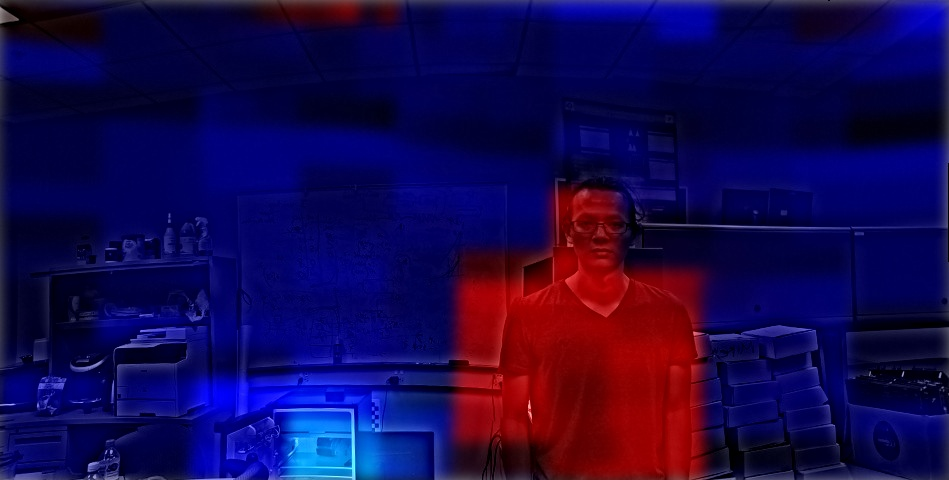
\epsfig{file=Exp0.jpg,height=1.5in,width=2.5in}
\end{center}
\end{minipage}
\begin{minipage}{1.2\textwidth}
\begin{center}

\epsfig{file=IRsttich.jpg,height=1.5in,width=2.5in }
\end{center}
\end{minipage}
\caption{Stitched Image: Fridge and Human body}
\label{fig:Stitched}
\end{figure*}
 


\subsection{Experiment 2: Discerning Two Human bodies and an Open Fridge}
\subsection{Experiment 3: Discerning Two Human bodies and a Running Portable Heater}     
 
\subsection{Insights}

\section{Conclusion}	
%%%%%%%%%%%%%%%%%%%%%%%%%%%%%%%%%%%%%%%%%%%%%%%%%%%%%%%%%%%%%%%%%%%%%%%%%%%%%%%%%%%%%%%%%%%%%%%%%%%%%%%%%	
%%%%%%%%%%%%%%%%%%%%%%%%%%%%%%%%%%%%%%%%%%%%%%%%%%%%%%%%%%%%%%%%%%%%%%%%%%%%%%%%%%%%%%%%%%%%%%%%%%%%%%%%%
%%%%%%%%%%%%%%%%%%%%%%%%%%%%%%%%%%%%%%%%%%%%%%%%%%%%%%%%%%%%%%%%%%%%%%%%%%%%%%%%%%%%%%%%%%%%%%%%%%%%%%%%% 
%%%%%%%%%%%%%%%%%%%%%%%%%%%%%%%%%%%%%%%%%%%%%%%%%%%%%%%%%%%%%%%%%%%%%%%%%%%%%%%%%%%%%%%%%%%%%%%%%%%%%%%%%
%%%%%%%%%%%%%%%%%%%%%%%%%%%%%%%%%%%%%%%%%%%%%%%%%%%%%%%%%%%%%%%%%%%%%%%%%%%%%%%%%%%%%%%%%%%%%%%%%%%%%%%%%
%%%%%%%%%%%%%%%%%%%%%%%%%%%%%%%%%%%%%%%%%%%%%%%%%%%%%%%%%%%%%%%%%%%%%%%%%%%%%%%%%%%%%%%%%%%%%%%%%%%%%%%%%
 

\begin{thebibliography}{9}
\bibitem{Stitch}  Matthew Brown and David G. Lowe. 2007. Automatic Panoramic Image Stitching using Invariant Features. Int. J. Comput. Vision 74, 1 (August 2007), 59-73.

\bibitem{EIA2014} 
 EIA 2014  http://www.eia.gov/electricity/sales$\_$revenue$\_$price/pdf/table5$\_$a.pdf, 2014. 
       
\bibitem{SPOT} P. X. Gao and S. Keshav. SPOT: A Smart Personalized Office Thermal Control System. In Proc. ACM e-Energy 2013, 2013.

\bibitem{SPOT+} P. X. Gao and S. Keshav. Optimal Personal Comfort Management Using SPOT+. In Proceedings of the Fifth ACM Workshop on Embedded Systems For Energy-Efficient Buildings, pages 1-8. ACM, 2013. 

\bibitem{Otsu} M. Sezgin and B. Sankur. Survey over image thresholding techniques and quantitative performance evaluation. Journal of Electronic Imaging 13, 2004.

\end{thebibliography}
\end{document}